\documentclass[twoside]{book}

% Packages required by doxygen
\usepackage{fixltx2e}
\usepackage{calc}
\usepackage{doxygen}
\usepackage[export]{adjustbox} % also loads graphicx
\usepackage{graphicx}
\usepackage[utf8]{inputenc}
\usepackage{makeidx}
\usepackage{multicol}
\usepackage{multirow}
\PassOptionsToPackage{warn}{textcomp}
\usepackage{textcomp}
\usepackage[nointegrals]{wasysym}
\usepackage[table]{xcolor}

% Font selection
\usepackage[T1]{fontenc}
\usepackage[scaled=.90]{helvet}
\usepackage{courier}
\usepackage{amssymb}
\usepackage{sectsty}
\renewcommand{\familydefault}{\sfdefault}
\allsectionsfont{%
  \fontseries{bc}\selectfont%
  \color{darkgray}%
}
\renewcommand{\DoxyLabelFont}{%
  \fontseries{bc}\selectfont%
  \color{darkgray}%
}
\newcommand{\+}{\discretionary{\mbox{\scriptsize$\hookleftarrow$}}{}{}}

% Page & text layout
\usepackage{geometry}
\geometry{%
  a4paper,%
  top=2.5cm,%
  bottom=2.5cm,%
  left=2.5cm,%
  right=2.5cm%
}
\tolerance=750
\hfuzz=15pt
\hbadness=750
\setlength{\emergencystretch}{15pt}
\setlength{\parindent}{0cm}
\setlength{\parskip}{3ex plus 2ex minus 2ex}
\makeatletter
\renewcommand{\paragraph}{%
  \@startsection{paragraph}{4}{0ex}{-1.0ex}{1.0ex}{%
    \normalfont\normalsize\bfseries\SS@parafont%
  }%
}
\renewcommand{\subparagraph}{%
  \@startsection{subparagraph}{5}{0ex}{-1.0ex}{1.0ex}{%
    \normalfont\normalsize\bfseries\SS@subparafont%
  }%
}
\makeatother

% Headers & footers
\usepackage{fancyhdr}
\pagestyle{fancyplain}
\fancyhead[LE]{\fancyplain{}{\bfseries\thepage}}
\fancyhead[CE]{\fancyplain{}{}}
\fancyhead[RE]{\fancyplain{}{\bfseries\leftmark}}
\fancyhead[LO]{\fancyplain{}{\bfseries\rightmark}}
\fancyhead[CO]{\fancyplain{}{}}
\fancyhead[RO]{\fancyplain{}{\bfseries\thepage}}
\fancyfoot[LE]{\fancyplain{}{}}
\fancyfoot[CE]{\fancyplain{}{}}
\fancyfoot[RE]{\fancyplain{}{\bfseries\scriptsize Generated by Doxygen }}
\fancyfoot[LO]{\fancyplain{}{\bfseries\scriptsize Generated by Doxygen }}
\fancyfoot[CO]{\fancyplain{}{}}
\fancyfoot[RO]{\fancyplain{}{}}
\renewcommand{\footrulewidth}{0.4pt}
\renewcommand{\chaptermark}[1]{%
  \markboth{#1}{}%
}
\renewcommand{\sectionmark}[1]{%
  \markright{\thesection\ #1}%
}

% Indices & bibliography
\usepackage{natbib}
\usepackage[titles]{tocloft}
\setcounter{tocdepth}{3}
\setcounter{secnumdepth}{5}
\makeindex

% Hyperlinks (required, but should be loaded last)
\usepackage{ifpdf}
\ifpdf
  \usepackage[pdftex,pagebackref=true]{hyperref}
\else
  \usepackage[ps2pdf,pagebackref=true]{hyperref}
\fi
\hypersetup{%
  colorlinks=true,%
  linkcolor=blue,%
  citecolor=blue,%
  unicode%
}

% Custom commands
\newcommand{\clearemptydoublepage}{%
  \newpage{\pagestyle{empty}\cleardoublepage}%
}

\usepackage{caption}
\captionsetup{labelsep=space,justification=centering,font={bf},singlelinecheck=off,skip=4pt,position=top}

%===== C O N T E N T S =====

\begin{document}

% Titlepage & ToC
\hypersetup{pageanchor=false,
             bookmarksnumbered=true,
             pdfencoding=unicode
            }
\pagenumbering{alph}
\begin{titlepage}
\vspace*{7cm}
\begin{center}%
{\Large Ipass }\\
\vspace*{1cm}
{\large Generated by Doxygen 1.8.13}\\
\end{center}
\end{titlepage}
\clearemptydoublepage
\pagenumbering{roman}
\tableofcontents
\clearemptydoublepage
\pagenumbering{arabic}
\hypersetup{pageanchor=true}

%--- Begin generated contents ---
\chapter{Hierarchical Index}
\section{Class Hierarchy}
This inheritance list is sorted roughly, but not completely, alphabetically\+:\begin{DoxyCompactList}
\item \contentsline{section}{colorholder}{\pageref{classcolorholder}}{}
\item \contentsline{section}{display}{\pageref{classdisplay}}{}
\item port\+\_\+out\begin{DoxyCompactList}
\item \contentsline{section}{hwlib\+:\+:invert\+\_\+port\+\_\+out\+\_\+from\+\_\+pins}{\pageref{classhwlib_1_1invert__port__out__from__pins}}{}
\end{DoxyCompactList}
\item \contentsline{section}{punt}{\pageref{classpunt}}{}
\end{DoxyCompactList}

\chapter{Class Index}
\section{Class List}
Here are the classes, structs, unions and interfaces with brief descriptions\+:\begin{DoxyCompactList}
\item\contentsline{section}{\hyperlink{classcolorholder}{colorholder} }{\pageref{classcolorholder}}{}
\item\contentsline{section}{\hyperlink{classdisplay}{display} }{\pageref{classdisplay}}{}
\item\contentsline{section}{\hyperlink{classhwlib_1_1invert__port__out__from__pins}{hwlib\+::invert\+\_\+port\+\_\+out\+\_\+from\+\_\+pins} }{\pageref{classhwlib_1_1invert__port__out__from__pins}}{}
\item\contentsline{section}{\hyperlink{classpunt}{punt} }{\pageref{classpunt}}{}
\end{DoxyCompactList}

\chapter{Class Documentation}
\hypertarget{classcolorholder}{}\section{colorholder Class Reference}
\label{classcolorholder}\index{colorholder@{colorholder}}
\subsection*{Public Member Functions}
\begin{DoxyCompactItemize}
\item 
\mbox{\Hypertarget{classcolorholder_a51a5abd7f56d8c917e4860b72c9d4b01}\label{classcolorholder_a51a5abd7f56d8c917e4860b72c9d4b01}} 
{\bfseries colorholder} (int color1=0, int color2=0)
\item 
\mbox{\Hypertarget{classcolorholder_a6630ad90e4100b213b98f8e0fe8ebf59}\label{classcolorholder_a6630ad90e4100b213b98f8e0fe8ebf59}} 
int {\bfseries getcolor1} ()
\item 
\mbox{\Hypertarget{classcolorholder_a67fd6b9bb75b098f42205bbdd004efb6}\label{classcolorholder_a67fd6b9bb75b098f42205bbdd004efb6}} 
int {\bfseries getcolor2} ()
\end{DoxyCompactItemize}


The documentation for this class was generated from the following file\+:\begin{DoxyCompactItemize}
\item 
colorholder.\+hpp\end{DoxyCompactItemize}

\hypertarget{classdisplay}{}\section{display Class Reference}
\label{classdisplay}\index{display@{display}}
\subsection*{Public Member Functions}
\begin{DoxyCompactItemize}
\item 
\mbox{\Hypertarget{classdisplay_a0425b78e4b91c1e1dcfa22f899787ce8}\label{classdisplay_a0425b78e4b91c1e1dcfa22f899787ce8}} 
{\bfseries display} (hwlib\+::target\+::pin\+\_\+out \&db0, hwlib\+::target\+::pin\+\_\+out \&db1, hwlib\+::target\+::pin\+\_\+out \&db2, hwlib\+::target\+::pin\+\_\+out \&db3, hwlib\+::target\+::pin\+\_\+out \&db4, hwlib\+::target\+::pin\+\_\+out \&db5, hwlib\+::target\+::pin\+\_\+out \&db6, hwlib\+::target\+::pin\+\_\+out \&db7, hwlib\+::target\+::pin\+\_\+out \&db8, hwlib\+::target\+::pin\+\_\+out \&db9, hwlib\+::target\+::pin\+\_\+out \&db10, hwlib\+::target\+::pin\+\_\+out \&db11, hwlib\+::target\+::pin\+\_\+out \&db12, hwlib\+::target\+::pin\+\_\+out \&db13, hwlib\+::target\+::pin\+\_\+out \&db14, hwlib\+::target\+::pin\+\_\+out \&db15, hwlib\+::target\+::pin\+\_\+out \&rst, hwlib\+::target\+::pin\+\_\+out \&cs, hwlib\+::target\+::pin\+\_\+out \&rs, hwlib\+::target\+::pin\+\_\+out \&wr, hwlib\+::target\+::pin\+\_\+in \&T\+\_\+do, hwlib\+::target\+::pin\+\_\+out \&T\+\_\+clk, hwlib\+::target\+::pin\+\_\+out \&T\+\_\+cs, hwlib\+::target\+::pin\+\_\+out \&T\+\_\+din, hwlib\+::target\+::pin\+\_\+in \&T\+\_\+irq)
\item 
\mbox{\Hypertarget{classdisplay_aed272c6c723e2fd976d436e32807e1d5}\label{classdisplay_aed272c6c723e2fd976d436e32807e1d5}} 
void {\bfseries L\+C\+D\+\_\+write\+\_\+\+Bus} (uint16\+\_\+t data1)
\item 
\mbox{\Hypertarget{classdisplay_a3943c805196989ec323e74bb5a313e25}\label{classdisplay_a3943c805196989ec323e74bb5a313e25}} 
void \hyperlink{classdisplay_a3943c805196989ec323e74bb5a313e25}{clear} ()
\begin{DoxyCompactList}\small\item\em make\textquotesingle{}s the screen white \end{DoxyCompactList}\item 
\mbox{\Hypertarget{classdisplay_a65036271ee5031dcc04a9e53e013e5d4}\label{classdisplay_a65036271ee5031dcc04a9e53e013e5d4}} 
void \hyperlink{classdisplay_a65036271ee5031dcc04a9e53e013e5d4}{customclear} (int x0, int y0, int x1, int y1)
\begin{DoxyCompactList}\small\item\em clears the screen with custom coördinates \end{DoxyCompactList}\item 
void \hyperlink{classdisplay_a1975e05bb65cbfcf209ace9dbea7d660}{L\+C\+D\+\_\+\+Write\+\_\+\+C\+OM} (uint8\+\_\+t com)
\begin{DoxyCompactList}\small\item\em function sends command \end{DoxyCompactList}\item 
void \hyperlink{classdisplay_a60e7eb3a85be87ac2867608fd35c9a02}{drawline} (uint\+\_\+fast16\+\_\+t x0, uint\+\_\+fast16\+\_\+t y0, uint\+\_\+fast16\+\_\+t x1, uint\+\_\+fast16\+\_\+t y1)
\begin{DoxyCompactList}\small\item\em Line drawing function. \end{DoxyCompactList}\item 
void \hyperlink{classdisplay_ad4f6e4f332f7d296d0917cfeff271507}{clr\+XY} ()
\begin{DoxyCompactList}\small\item\em needed for initialization \end{DoxyCompactList}\item 
\mbox{\Hypertarget{classdisplay_a6798596733a6427286ed80a651ad7bf3}\label{classdisplay_a6798596733a6427286ed80a651ad7bf3}} 
void {\bfseries clr\+Scr} ()
\item 
void \hyperlink{classdisplay_aa0b94eb3cb43b47dc720542cf7d1da9b}{init} ()
\begin{DoxyCompactList}\small\item\em initializes the display \end{DoxyCompactList}\item 
void \hyperlink{classdisplay_aea3fc9645f5b6a097cafd2524b4dd0ee}{drawcircle} (int x0, int y0, int radius)
\begin{DoxyCompactList}\small\item\em cirle drawing algorithm \end{DoxyCompactList}\item 
int \hyperlink{classdisplay_aa25dc0f889ff19b65c51fe6b94872398}{map} (int x, int in\+\_\+min, int in\+\_\+max, int out\+\_\+min, int out\+\_\+max)
\begin{DoxyCompactList}\small\item\em map is standard arduino function to arrang numbers \end{DoxyCompactList}\item 
\mbox{\Hypertarget{classdisplay_a0bdd9b4e66175b07c5bdd303504c0da4}\label{classdisplay_a0bdd9b4e66175b07c5bdd303504c0da4}} 
void {\bfseries pincontrol} (auto pin, unsigned short status)
\item 
\hyperlink{classpunt}{punt} \hyperlink{classdisplay_a7e3b873f8b5fbd55cbe65862c18374b3}{Touchread} ()
\begin{DoxyCompactList}\small\item\em reads touch input \end{DoxyCompactList}\item 
int16\+\_\+t \hyperlink{classdisplay_ac198f10fa30850e9e3fa71b0dc0c1d73}{Read\+Axis} (int Axis)
\begin{DoxyCompactList}\small\item\em Chooses wich Axis to read. \end{DoxyCompactList}\item 
uint16\+\_\+t \hyperlink{classdisplay_a701815d7bc53a0eea5f3fd2e020c36ae}{Read\+Data} ()
\begin{DoxyCompactList}\small\item\em reads touch data \end{DoxyCompactList}\item 
void \hyperlink{classdisplay_a3da84c7e17070441111af326cc03217a}{Output\+Data} (uint8\+\_\+t Data)
\begin{DoxyCompactList}\small\item\em sends a command to touchcontroller \end{DoxyCompactList}\item 
void \hyperlink{classdisplay_ade81aa04a5c49aaf7a663b7e03ca5a36}{Address\+\_\+set} (unsigned int x1, unsigned int y1, unsigned int x2, unsigned int y2)
\begin{DoxyCompactList}\small\item\em sends pixel location \end{DoxyCompactList}\end{DoxyCompactItemize}
\textbf{ }\par
\begin{DoxyCompactItemize}
\item 
void \hyperlink{classdisplay_a11803b9582f7336d28f2dc69be19bcfe}{L\+C\+D\+\_\+write\+\_\+\+Bus} (uint8\+\_\+t data1, uint8\+\_\+t data2)
\begin{DoxyCompactList}\small\item\em sends data to display controller \end{DoxyCompactList}\end{DoxyCompactItemize}

\textbf{ }\par
\begin{DoxyCompactItemize}
\item 
\mbox{\Hypertarget{classdisplay_a39b50018876dfbf2beff6d43244456a2}\label{classdisplay_a39b50018876dfbf2beff6d43244456a2}} 
void {\bfseries draw\+Pixel} (int x, int y, uint8\+\_\+t color1, uint8\+\_\+t color2)
\item 
\mbox{\Hypertarget{classdisplay_a9ed4ea04ea86be2c4e0ad21b2c8da0e1}\label{classdisplay_a9ed4ea04ea86be2c4e0ad21b2c8da0e1}} 
void {\bfseries draw\+Pixel} (int x, int y, uint16\+\_\+t color)
\item 
void \hyperlink{classdisplay_aafdae0e6f1d077e74c362ce0bd3124c9}{draw\+Pixel} (int x, int y)
\begin{DoxyCompactList}\small\item\em drawspixels for functions. \end{DoxyCompactList}\end{DoxyCompactItemize}

\textbf{ }\par
\begin{DoxyCompactItemize}
\item 
\mbox{\Hypertarget{classdisplay_a45b31b92e29b323031e21a0134614e70}\label{classdisplay_a45b31b92e29b323031e21a0134614e70}} 
void {\bfseries drawsingel\+Pixel} (int x, int y, uint8\+\_\+t color1, uint8\+\_\+t color2)
\item 
\mbox{\Hypertarget{classdisplay_a7922a61962bdf9b768119ee87cead4db}\label{classdisplay_a7922a61962bdf9b768119ee87cead4db}} 
void {\bfseries drawsingel\+Pixel} (int x, int y, uint16\+\_\+t color)
\item 
void \hyperlink{classdisplay_a33c1025dac3f51844cbb2c2cc191ad16}{drawsingel\+Pixel} (int x, int y)
\begin{DoxyCompactList}\small\item\em draws a single pixel \end{DoxyCompactList}\end{DoxyCompactItemize}

\textbf{ }\par
\begin{DoxyCompactItemize}
\item 
void \hyperlink{classdisplay_ae33f12ec551d199f3422a581fa40385c}{fillrect} (int x0, int y0, int x1, int y1, uint16\+\_\+t color)
\begin{DoxyCompactList}\small\item\em draws a filled rectangle \end{DoxyCompactList}\item 
\mbox{\Hypertarget{classdisplay_a85b1866b6bfc88a8f057052a5e8c09b9}\label{classdisplay_a85b1866b6bfc88a8f057052a5e8c09b9}} 
void {\bfseries fillrect} (int x0, int y0, int x1, int y1, uint8\+\_\+t color1, uint8\+\_\+t color2)
\end{DoxyCompactItemize}

\textbf{ }\par
{\em function sends pixel data

L\+C\+D\+\_\+\+Write\+\_\+\+D\+A\+TA

this function is used to send 8 or 16 bit pixel data to the display controller }\begin{DoxyCompactItemize}
\item 
\mbox{\Hypertarget{classdisplay_a459e32125fb569af6a22305413ea899a}\label{classdisplay_a459e32125fb569af6a22305413ea899a}} 
void {\bfseries L\+C\+D\+\_\+\+Write\+\_\+\+D\+A\+TA} (uint8\+\_\+t data1, uint8\+\_\+t data2)
\item 
\mbox{\Hypertarget{classdisplay_a03a6769063c17f2f22bd1b75bf1d5935}\label{classdisplay_a03a6769063c17f2f22bd1b75bf1d5935}} 
void {\bfseries L\+C\+D\+\_\+\+Write\+\_\+\+D\+A\+TA} (uint8\+\_\+t data1)
\end{DoxyCompactItemize}

\subsection*{Public Attributes}
\begin{DoxyCompactItemize}
\item 
\mbox{\Hypertarget{classdisplay_ab6b90d0b3f74bc8ccb379bba67457004}\label{classdisplay_ab6b90d0b3f74bc8ccb379bba67457004}} 
int {\bfseries drawcolor1} = 0x00
\item 
\mbox{\Hypertarget{classdisplay_a8f805030a8fb7876eda55bd1897db703}\label{classdisplay_a8f805030a8fb7876eda55bd1897db703}} 
int {\bfseries drawcolor2} = 0x00
\end{DoxyCompactItemize}


\subsection{Member Function Documentation}
\mbox{\Hypertarget{classdisplay_ade81aa04a5c49aaf7a663b7e03ca5a36}\label{classdisplay_ade81aa04a5c49aaf7a663b7e03ca5a36}} 
\index{display@{display}!Address\+\_\+set@{Address\+\_\+set}}
\index{Address\+\_\+set@{Address\+\_\+set}!display@{display}}
\subsubsection{\texorpdfstring{Address\+\_\+set()}{Address\_set()}}
{\footnotesize\ttfamily void display\+::\+Address\+\_\+set (\begin{DoxyParamCaption}\item[{unsigned int}]{x1,  }\item[{unsigned int}]{y1,  }\item[{unsigned int}]{x2,  }\item[{unsigned int}]{y2 }\end{DoxyParamCaption})}



sends pixel location 

sends pixel data two places in the memory \mbox{\Hypertarget{classdisplay_ad4f6e4f332f7d296d0917cfeff271507}\label{classdisplay_ad4f6e4f332f7d296d0917cfeff271507}} 
\index{display@{display}!clr\+XY@{clr\+XY}}
\index{clr\+XY@{clr\+XY}!display@{display}}
\subsubsection{\texorpdfstring{clr\+X\+Y()}{clrXY()}}
{\footnotesize\ttfamily void display\+::clr\+XY (\begin{DoxyParamCaption}{ }\end{DoxyParamCaption})}



needed for initialization 

sets the screensize \mbox{\Hypertarget{classdisplay_aea3fc9645f5b6a097cafd2524b4dd0ee}\label{classdisplay_aea3fc9645f5b6a097cafd2524b4dd0ee}} 
\index{display@{display}!drawcircle@{drawcircle}}
\index{drawcircle@{drawcircle}!display@{display}}
\subsubsection{\texorpdfstring{drawcircle()}{drawcircle()}}
{\footnotesize\ttfamily void display\+::drawcircle (\begin{DoxyParamCaption}\item[{int}]{x0,  }\item[{int}]{y0,  }\item[{int}]{radius }\end{DoxyParamCaption})}



cirle drawing algorithm 

An alogrithm from wikipedia same as hwlib thats draws circle based on x and y cordinate \mbox{\Hypertarget{classdisplay_a60e7eb3a85be87ac2867608fd35c9a02}\label{classdisplay_a60e7eb3a85be87ac2867608fd35c9a02}} 
\index{display@{display}!drawline@{drawline}}
\index{drawline@{drawline}!display@{display}}
\subsubsection{\texorpdfstring{drawline()}{drawline()}}
{\footnotesize\ttfamily void display\+::drawline (\begin{DoxyParamCaption}\item[{uint\+\_\+fast16\+\_\+t}]{x0,  }\item[{uint\+\_\+fast16\+\_\+t}]{y0,  }\item[{uint\+\_\+fast16\+\_\+t}]{x1,  }\item[{uint\+\_\+fast16\+\_\+t}]{y1 }\end{DoxyParamCaption})}



Line drawing function. 

This function draws lines from one point to another on lcd screen alogrothim used from website below \href{http://c.happycodings.com/games-and-graphics/code18.html}{\tt http\+://c.\+happycodings.\+com/games-\/and-\/graphics/code18.\+html} \mbox{\Hypertarget{classdisplay_aafdae0e6f1d077e74c362ce0bd3124c9}\label{classdisplay_aafdae0e6f1d077e74c362ce0bd3124c9}} 
\index{display@{display}!draw\+Pixel@{draw\+Pixel}}
\index{draw\+Pixel@{draw\+Pixel}!display@{display}}
\subsubsection{\texorpdfstring{draw\+Pixel()}{drawPixel()}}
{\footnotesize\ttfamily void display\+::draw\+Pixel (\begin{DoxyParamCaption}\item[{int}]{x,  }\item[{int}]{y }\end{DoxyParamCaption})}



drawspixels for functions. 

This drawpixel is for drawing multiple pixels after each other this one leaves the chipselect high to speed up the process if you dont pass a color it prins black pixels you can pass 8bit or 16 bit color 16 bit color can been sent in 8 bit format or 16 bit format \mbox{\Hypertarget{classdisplay_a33c1025dac3f51844cbb2c2cc191ad16}\label{classdisplay_a33c1025dac3f51844cbb2c2cc191ad16}} 
\index{display@{display}!drawsingel\+Pixel@{drawsingel\+Pixel}}
\index{drawsingel\+Pixel@{drawsingel\+Pixel}!display@{display}}
\subsubsection{\texorpdfstring{drawsingel\+Pixel()}{drawsingelPixel()}}
{\footnotesize\ttfamily void display\+::drawsingel\+Pixel (\begin{DoxyParamCaption}\item[{int}]{x,  }\item[{int}]{y }\end{DoxyParamCaption})}



draws a single pixel 

draws a single pixel if you dont pass a color it prins black pixels you can pass 8bit or 16 bit color 16 bit color can been sent in 8 bit format or 16 bit format \mbox{\Hypertarget{classdisplay_ae33f12ec551d199f3422a581fa40385c}\label{classdisplay_ae33f12ec551d199f3422a581fa40385c}} 
\index{display@{display}!fillrect@{fillrect}}
\index{fillrect@{fillrect}!display@{display}}
\subsubsection{\texorpdfstring{fillrect()}{fillrect()}}
{\footnotesize\ttfamily void display\+::fillrect (\begin{DoxyParamCaption}\item[{int}]{x0,  }\item[{int}]{y0,  }\item[{int}]{x1,  }\item[{int}]{y1,  }\item[{uint16\+\_\+t}]{color }\end{DoxyParamCaption})}



draws a filled rectangle 

draws filled rectangle in the color of choice \mbox{\Hypertarget{classdisplay_aa0b94eb3cb43b47dc720542cf7d1da9b}\label{classdisplay_aa0b94eb3cb43b47dc720542cf7d1da9b}} 
\index{display@{display}!init@{init}}
\index{init@{init}!display@{display}}
\subsubsection{\texorpdfstring{init()}{init()}}
{\footnotesize\ttfamily void display\+::init (\begin{DoxyParamCaption}{ }\end{DoxyParamCaption})}



initializes the display 

reset the display and initializes a the display commands are copyed from utft libary \mbox{\Hypertarget{classdisplay_a11803b9582f7336d28f2dc69be19bcfe}\label{classdisplay_a11803b9582f7336d28f2dc69be19bcfe}} 
\index{display@{display}!L\+C\+D\+\_\+write\+\_\+\+Bus@{L\+C\+D\+\_\+write\+\_\+\+Bus}}
\index{L\+C\+D\+\_\+write\+\_\+\+Bus@{L\+C\+D\+\_\+write\+\_\+\+Bus}!display@{display}}
\subsubsection{\texorpdfstring{L\+C\+D\+\_\+write\+\_\+\+Bus()}{LCD\_write\_Bus()}}
{\footnotesize\ttfamily void display\+::\+L\+C\+D\+\_\+write\+\_\+\+Bus (\begin{DoxyParamCaption}\item[{uint8\+\_\+t}]{data1,  }\item[{uint8\+\_\+t}]{data2 }\end{DoxyParamCaption})}



sends data to display controller 

sends data to display in 16 bit format in two 8 bit loops also supports 16bit color format \mbox{\Hypertarget{classdisplay_a1975e05bb65cbfcf209ace9dbea7d660}\label{classdisplay_a1975e05bb65cbfcf209ace9dbea7d660}} 
\index{display@{display}!L\+C\+D\+\_\+\+Write\+\_\+\+C\+OM@{L\+C\+D\+\_\+\+Write\+\_\+\+C\+OM}}
\index{L\+C\+D\+\_\+\+Write\+\_\+\+C\+OM@{L\+C\+D\+\_\+\+Write\+\_\+\+C\+OM}!display@{display}}
\subsubsection{\texorpdfstring{L\+C\+D\+\_\+\+Write\+\_\+\+C\+O\+M()}{LCD\_Write\_COM()}}
{\footnotesize\ttfamily void display\+::\+L\+C\+D\+\_\+\+Write\+\_\+\+C\+OM (\begin{DoxyParamCaption}\item[{uint8\+\_\+t}]{com }\end{DoxyParamCaption})}



function sends command 

this function is used to send command to the display controller \mbox{\Hypertarget{classdisplay_aa25dc0f889ff19b65c51fe6b94872398}\label{classdisplay_aa25dc0f889ff19b65c51fe6b94872398}} 
\index{display@{display}!map@{map}}
\index{map@{map}!display@{display}}
\subsubsection{\texorpdfstring{map()}{map()}}
{\footnotesize\ttfamily int display\+::map (\begin{DoxyParamCaption}\item[{int}]{x,  }\item[{int}]{in\+\_\+min,  }\item[{int}]{in\+\_\+max,  }\item[{int}]{out\+\_\+min,  }\item[{int}]{out\+\_\+max }\end{DoxyParamCaption})}



map is standard arduino function to arrang numbers 

it re-\/maps a number from one range to another \mbox{\Hypertarget{classdisplay_a3da84c7e17070441111af326cc03217a}\label{classdisplay_a3da84c7e17070441111af326cc03217a}} 
\index{display@{display}!Output\+Data@{Output\+Data}}
\index{Output\+Data@{Output\+Data}!display@{display}}
\subsubsection{\texorpdfstring{Output\+Data()}{OutputData()}}
{\footnotesize\ttfamily void display\+::\+Output\+Data (\begin{DoxyParamCaption}\item[{uint8\+\_\+t}]{Data }\end{DoxyParamCaption})}



sends a command to touchcontroller 

sends a 8 bit command to touch conrtroller uses a clockvoid \hyperlink{classdisplay_a3da84c7e17070441111af326cc03217a}{display\+::\+Output\+Data(uint8\+\_\+t Data)} \mbox{\Hypertarget{classdisplay_ac198f10fa30850e9e3fa71b0dc0c1d73}\label{classdisplay_ac198f10fa30850e9e3fa71b0dc0c1d73}} 
\index{display@{display}!Read\+Axis@{Read\+Axis}}
\index{Read\+Axis@{Read\+Axis}!display@{display}}
\subsubsection{\texorpdfstring{Read\+Axis()}{ReadAxis()}}
{\footnotesize\ttfamily int16\+\_\+t display\+::\+Read\+Axis (\begin{DoxyParamCaption}\item[{int}]{Axis }\end{DoxyParamCaption})}



Chooses wich Axis to read. 

Send command to the touch controller if it want to read X or Y Axis then it sets clock pulse and starts the read data function \mbox{\Hypertarget{classdisplay_a701815d7bc53a0eea5f3fd2e020c36ae}\label{classdisplay_a701815d7bc53a0eea5f3fd2e020c36ae}} 
\index{display@{display}!Read\+Data@{Read\+Data}}
\index{Read\+Data@{Read\+Data}!display@{display}}
\subsubsection{\texorpdfstring{Read\+Data()}{ReadData()}}
{\footnotesize\ttfamily uint16\+\_\+t display\+::\+Read\+Data (\begin{DoxyParamCaption}\item[{void}]{ }\end{DoxyParamCaption})}



reads touch data 

reads touch data from the data line on basis of a clock line \mbox{\Hypertarget{classdisplay_a7e3b873f8b5fbd55cbe65862c18374b3}\label{classdisplay_a7e3b873f8b5fbd55cbe65862c18374b3}} 
\index{display@{display}!Touchread@{Touchread}}
\index{Touchread@{Touchread}!display@{display}}
\subsubsection{\texorpdfstring{Touchread()}{Touchread()}}
{\footnotesize\ttfamily \hyperlink{classpunt}{punt} display\+::\+Touchread (\begin{DoxyParamCaption}{ }\end{DoxyParamCaption})}



reads touch input 

reads touch input and preforms a few checks if its a valid coördinate 

The documentation for this class was generated from the following files\+:\begin{DoxyCompactItemize}
\item 
display.\+hpp\item 
display.\+cpp\end{DoxyCompactItemize}

\hypertarget{classhwlib_1_1invert__port__out__from__pins}{}\section{hwlib\+:\+:invert\+\_\+port\+\_\+out\+\_\+from\+\_\+pins Class Reference}
\label{classhwlib_1_1invert__port__out__from__pins}\index{hwlib\+::invert\+\_\+port\+\_\+out\+\_\+from\+\_\+pins@{hwlib\+::invert\+\_\+port\+\_\+out\+\_\+from\+\_\+pins}}
Inheritance diagram for hwlib\+:\+:invert\+\_\+port\+\_\+out\+\_\+from\+\_\+pins\+:\begin{figure}[H]
\begin{center}
\leavevmode
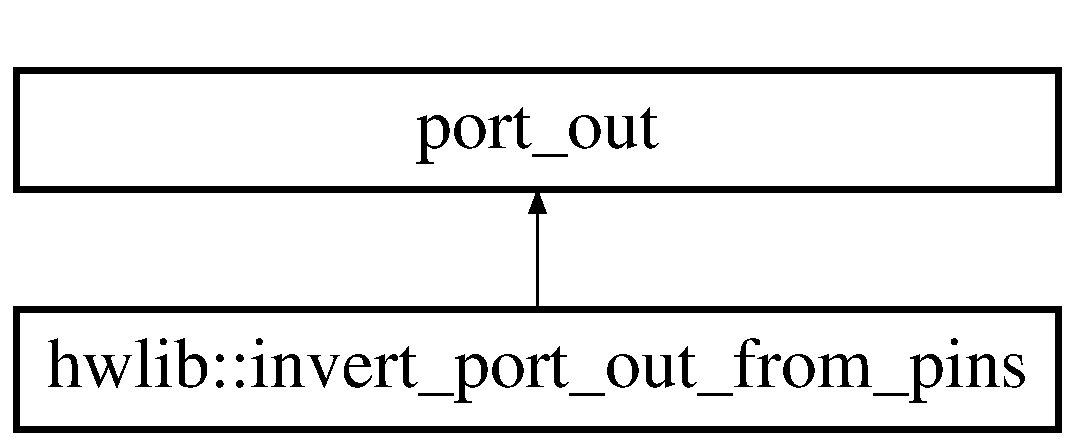
\includegraphics[height=2.000000cm]{classhwlib_1_1invert__port__out__from__pins}
\end{center}
\end{figure}
\subsection*{Public Member Functions}
\begin{DoxyCompactItemize}
\item 
\hyperlink{classhwlib_1_1invert__port__out__from__pins_a2eae53fe915f8e09ab5d66594d79ef29}{invert\+\_\+port\+\_\+out\+\_\+from\+\_\+pins} (pin\+\_\+out \&p0=pin\+\_\+out\+\_\+dummy, pin\+\_\+out \&p1=pin\+\_\+out\+\_\+dummy, pin\+\_\+out \&p2=pin\+\_\+out\+\_\+dummy, pin\+\_\+out \&p3=pin\+\_\+out\+\_\+dummy, pin\+\_\+out \&p4=pin\+\_\+out\+\_\+dummy, pin\+\_\+out \&p5=pin\+\_\+out\+\_\+dummy, pin\+\_\+out \&p6=pin\+\_\+out\+\_\+dummy, pin\+\_\+out \&p7=pin\+\_\+out\+\_\+dummy)
\begin{DoxyCompactList}\small\item\em construct a port\+\_\+out from up to 16 pin\+\_\+outs \end{DoxyCompactList}\item 
\mbox{\Hypertarget{classhwlib_1_1invert__port__out__from__pins_a4337f4b89402a5cf359d682cecdeb349}\label{classhwlib_1_1invert__port__out__from__pins_a4337f4b89402a5cf359d682cecdeb349}} 
uint\+\_\+fast8\+\_\+t {\bfseries number\+\_\+of\+\_\+pins} () override
\item 
\mbox{\Hypertarget{classhwlib_1_1invert__port__out__from__pins_a05fbc97458115a8413dc2739449d755f}\label{classhwlib_1_1invert__port__out__from__pins_a05fbc97458115a8413dc2739449d755f}} 
void {\bfseries set} (uint\+\_\+fast8\+\_\+t x, buffering buf=buffering\+::unbuffered) override
\end{DoxyCompactItemize}


\subsection{Constructor \& Destructor Documentation}
\mbox{\Hypertarget{classhwlib_1_1invert__port__out__from__pins_a2eae53fe915f8e09ab5d66594d79ef29}\label{classhwlib_1_1invert__port__out__from__pins_a2eae53fe915f8e09ab5d66594d79ef29}} 
\index{hwlib\+::invert\+\_\+port\+\_\+out\+\_\+from\+\_\+pins@{hwlib\+::invert\+\_\+port\+\_\+out\+\_\+from\+\_\+pins}!invert\+\_\+port\+\_\+out\+\_\+from\+\_\+pins@{invert\+\_\+port\+\_\+out\+\_\+from\+\_\+pins}}
\index{invert\+\_\+port\+\_\+out\+\_\+from\+\_\+pins@{invert\+\_\+port\+\_\+out\+\_\+from\+\_\+pins}!hwlib\+::invert\+\_\+port\+\_\+out\+\_\+from\+\_\+pins@{hwlib\+::invert\+\_\+port\+\_\+out\+\_\+from\+\_\+pins}}
\subsubsection{\texorpdfstring{invert\+\_\+port\+\_\+out\+\_\+from\+\_\+pins()}{invert\_port\_out\_from\_pins()}}
{\footnotesize\ttfamily hwlib\+::invert\+\_\+port\+\_\+out\+\_\+from\+\_\+pins\+::invert\+\_\+port\+\_\+out\+\_\+from\+\_\+pins (\begin{DoxyParamCaption}\item[{pin\+\_\+out \&}]{p0 = {\ttfamily pin\+\_\+out\+\_\+dummy},  }\item[{pin\+\_\+out \&}]{p1 = {\ttfamily pin\+\_\+out\+\_\+dummy},  }\item[{pin\+\_\+out \&}]{p2 = {\ttfamily pin\+\_\+out\+\_\+dummy},  }\item[{pin\+\_\+out \&}]{p3 = {\ttfamily pin\+\_\+out\+\_\+dummy},  }\item[{pin\+\_\+out \&}]{p4 = {\ttfamily pin\+\_\+out\+\_\+dummy},  }\item[{pin\+\_\+out \&}]{p5 = {\ttfamily pin\+\_\+out\+\_\+dummy},  }\item[{pin\+\_\+out \&}]{p6 = {\ttfamily pin\+\_\+out\+\_\+dummy},  }\item[{pin\+\_\+out \&}]{p7 = {\ttfamily pin\+\_\+out\+\_\+dummy} }\end{DoxyParamCaption})\hspace{0.3cm}{\ttfamily [inline]}}



construct a port\+\_\+out from up to 16 pin\+\_\+outs 

This constructor creates a port\+\_\+out from up to 8 pin\+\_\+out pins. The first pin is the lowest pin in the port, etc. 

The documentation for this class was generated from the following file\+:\begin{DoxyCompactItemize}
\item 
display.\+cpp\end{DoxyCompactItemize}

\hypertarget{classpunt}{}\section{punt Class Reference}
\label{classpunt}\index{punt@{punt}}
\subsection*{Public Member Functions}
\begin{DoxyCompactItemize}
\item 
\mbox{\Hypertarget{classpunt_a9c0b4caf91ddfacf516d561ccf74a38e}\label{classpunt_a9c0b4caf91ddfacf516d561ccf74a38e}} 
{\bfseries punt} (int x=0, int y=0)
\item 
\mbox{\Hypertarget{classpunt_aa1cae250f29ca9b72a9de0d560ea9518}\label{classpunt_aa1cae250f29ca9b72a9de0d560ea9518}} 
int {\bfseries getx} ()
\item 
\mbox{\Hypertarget{classpunt_a71869b9db737692169ed25fe04a7f935}\label{classpunt_a71869b9db737692169ed25fe04a7f935}} 
int {\bfseries gety} ()
\end{DoxyCompactItemize}


The documentation for this class was generated from the following file\+:\begin{DoxyCompactItemize}
\item 
punt.\+hpp\end{DoxyCompactItemize}

%--- End generated contents ---

% Index
\backmatter
\newpage
\phantomsection
\clearemptydoublepage
\addcontentsline{toc}{chapter}{Index}
\printindex

\end{document}
